\documentclass[openright,10pt,onecolumn]{report}

% % % Packages
\usepackage{afterpage}
\usepackage{sectsty}
% citation
\usepackage[noadjust]{cite}
% header and footer
\usepackage[english]{babel}
\usepackage[utf8]{inputenc}
\usepackage{fancyhdr}
\usepackage[table,xcdraw]{xcolor}
\usepackage{url}
\usepackage{multicol}

\usepackage[hyperfootnotes=false]{hyperref}
%cross reference
\usepackage{hyperref}
\hypersetup{
    colorlinks=true,
    linkcolor=black,
    hyperfootnotes = false,
    filecolor=magenta,      
    urlcolor=cyan,
    pdftitle={Sharelatex Example},
    bookmarks=true,
    pdfpagemode=FullScreen,
    citecolor=black
}

%caption
\usepackage{caption} 
\captionsetup[table]{skip=2pt}

% Margin configuration

%geometry of main textbook
\usepackage[left=2cm, right=2cm, top=3cm , bottom=3cm , headsep=.75cm , voffset =.55cm]{geometry}

\usepackage{algorithm}
\usepackage{pseudocode}
\renewcommand\headrulewidth{1.5pt}

% Header and footer configuration
\pagestyle{fancy}

\renewcommand{\chaptername}{}
\renewcommand{\chaptermark}[1]{%
\markboth{#1}{}}
\renewcommand{\sectionmark}[1]{\markright{\thesubsection\ #1}}

\fancyhf{}
\fancyhead[RO]{\begin{picture}(0,0) \put(-75,0){\includegraphics[width=3.4cm]{Team_Logo}} \end{picture}}
\lhead{\large\nouppercase{\leftmark}}
\cfoot{\thepage}

\usepackage[pdftex]{graphicx}
\usepackage{subcaption}
\usepackage{indentfirst}
\usepackage{tikz}
\usepackage{tabularx,booktabs}
\newcolumntype{C}{>{\centering\arraybackslash}X} % centered version of "X" type
\setlength{\extrarowheight}{1pt}
\usepackage{lipsum}
\usetikzlibrary{shapes,arrows}
\usepackage[export]{adjustbox}

\usepackage{mwe}
\usepackage{float}
\usepackage{amssymb}
\usepackage{arydshln}
\usepackage{amsmath}
\usepackage{booktabs,siunitx,multirow,enumitem,tabularx}
\usepackage{pifont}% http://ctan.org/pkg/pifont
\newcommand{\chmark}{\ding{51}}%
\newcommand{\xmark}{\ding{55}}%
\usepackage{tasks}
\usepackage{exsheets}
\usepackage{color,soul}
\usepackage{wrapfig, blindtext}
\usepackage{pdfpages}
\usepackage{xparse} 

% Acronyms
\usepackage{acronym}
% % Acronym list

% creat your acronym like this
% \newacronym{dsg}{DSG}{Deep Space Gateway}
% then insert this before end{document}
% \printglossary[title={Acronym},type=\acronymtype,nonumberlist]



% Set line spacing
\usepackage{setspace}

% Configuration for title
\usepackage{titlesec}
%%%\newcommand{\bigrule}{\titlerule[0.5mm]}
%%%\renewcommand{\rmdefault}{bch} 
\titleformat{\chapter}[display]
{\normalfont}{}
{0pt}{\LARGE\bfseries}                      %left/raght %up/down 
\titlespacing*{\chapter} {0pt}{-30pt}{5pt}
\titlespacing*{\section} {0pt}{-3pt}{3pt}
\titlespacing*{\subsection} {0pt}{-1pt}{3pt}
\titlespacing*{\subsubsection} {0pt}{-1pt}{3pt}


%header and footer in chapter page
\usepackage{etoolbox}
\makeatletter
\let\ps@plain\ps@fancy
\makeatother
%Reference name
\makeatletter
\def\thebibliography#1{\chapter*{References\@mkboth
  {REFERENCES}{REFERENCES}}\list
  {[\arabic{enumi}]}{\settowidth\labelwidth{[#1]}\leftmargin\labelwidth
\advance\leftmargin\labelsep
\usecounter{enumi}}
\def\newblock{\hskip .81em plus .93em minus .07em}
\sloppy\clubpenalty4000\widowpenalty4000
\sfcode`\.=1000\relax}
\makeatother

\renewcommand{\listfigurename}{List of Figures}
\renewcommand{\listtablename}{List of Tables}

\setcounter{tocdepth}{1}
%\setlength{\parskip}{1em}
%\setlength{\fboxsep}{0pt}




%\voffset = 15pt
%\headsep = 25pt

%%%%% main file
\begin{document}
\LARGE
%%%%% First page

\thispagestyle{empty}
\begin{centering}

 %\begin{figure}    
  %   \centering
   %  {\includegraphics[width=0.5\textwidth]{Team_Logo1}}
 %\end{figure}

  {\color{white}AIAA 2018-2019 Undergraduate Space System Design Competition}
  \begin{center}
    {\color{white}\line(1,0){470}} 
   \end{center}
   
  {\color{white}Submitted by}\\
 
  {\color{white}Sharif University Team: ShadX New Horizon}
  \begin{center}
    {\color{white}\line(1,0){470}} 
   \end{center}
     
  \begin{figure}[hbtp]   
    \centering
    {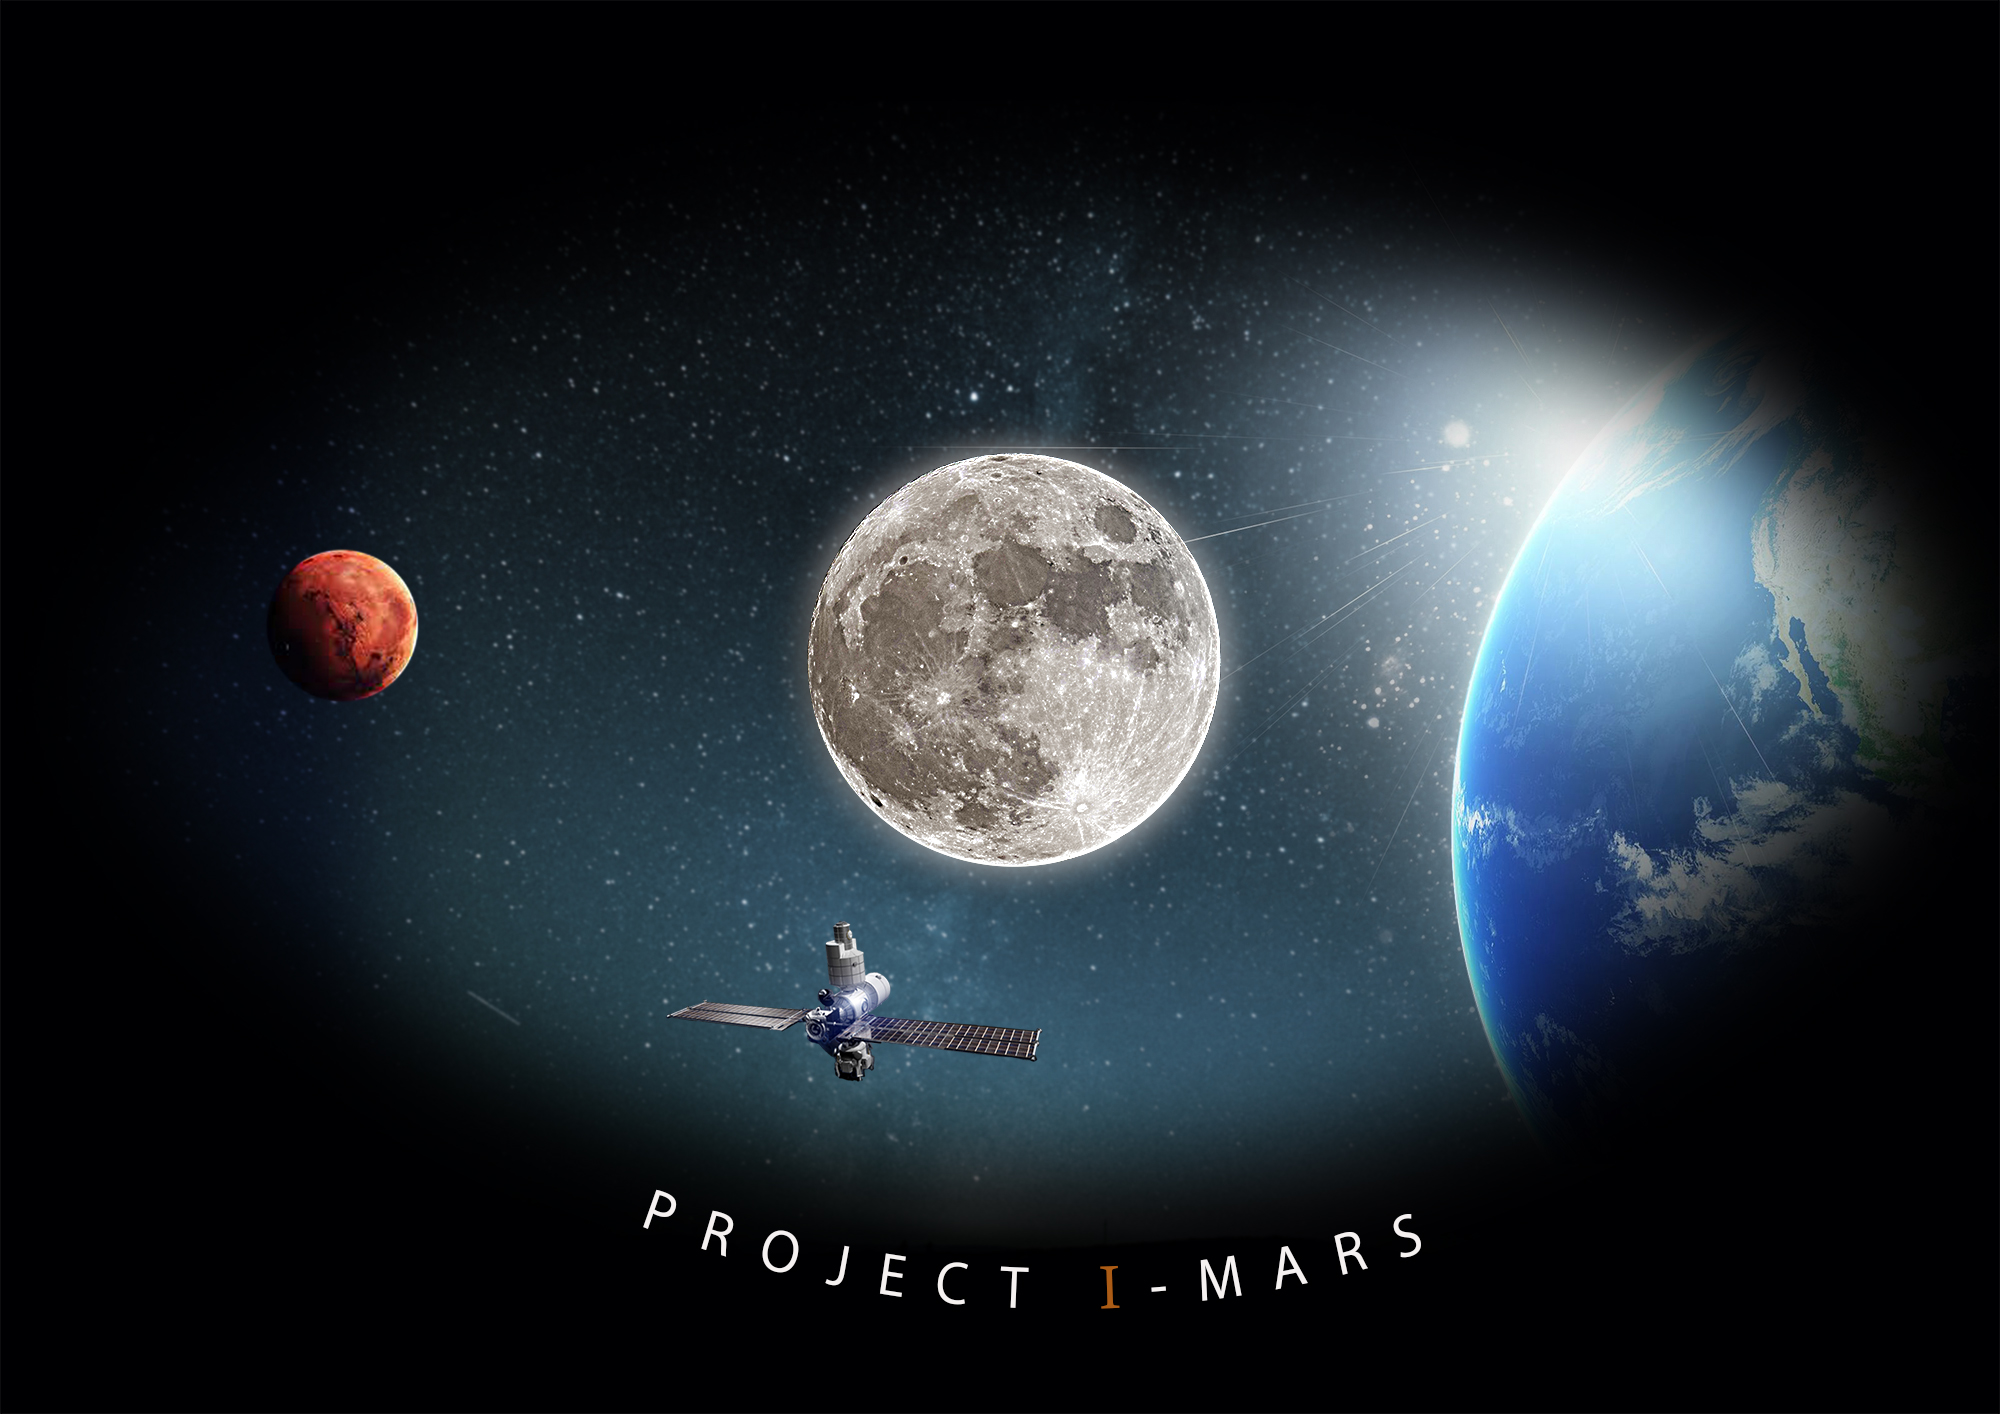
\includegraphics[width=\linewidth]{First_page}}
  \end{figure}
  \pagecolor{black}\afterpage{\nopagecolor}
  
  
  {\color{white}\textbf{Intelligent Multi surface Access Reusable Spacecraft}}\\
  
  {\color{white}\today}  

\end{centering}

%% Acknowledgments


\normalsize
\newpage%avoid page numbering in first page
%Contents
\pagenumbering{roman}

\newpage
\singlespacing

\renewcommand{\contentsname}{Table of Contents}

\begin{multicols}{2}
  \tableofcontents
\end{multicols}

\begin{multicols}{2}
\listoffigures
\end{multicols}

\addcontentsline{toc}{chapter}{List of Figures}
\begin{multicols}{2}
\listoftables
\end{multicols}

\addcontentsline{toc}{chapter}{List of Tables}
\afterpage{%
\newgeometry{left=2cm, right=2cm, top=2.7cm , bottom=2.7cm , headsep=1.25cm , voffset =1.25cm}

\twocolumn
\let\oldleftmark=\leftmark
\chapter*{Acronyms}
\renewcommand{\leftmark}{Acronyms}
\addcontentsline{toc}{chapter}{Acronyms}
\begin{acronym}

  \acro{ADCS}{Attitude Determination and Control System}
  \acro{AIAA}{American Institute of Aeronautics \\ and Astronautics}
  \acro{ATA}{Annular Tank Arrangement}
  \acro{AMPS}{Ariana Main Propulsion System}
  \acro{BEAM}{Bigelow Expanding Activity Module}
  \acro{BFR}{Big Falcon Rocket}
  \acro{BOL}{Beginning of Life}
  \acro{bps}{bits per second}
  \acro{BWG}{Beam waveguide antenna}
  \acro{CAD}{Computer Aided Design}
  \acro{CDH}{Command and Data Handling}
  \acro{CFRC}{Carbon Fiber Reinforced Carbon}
  \acro{CM}{Crew Member}
  \acro{CMG}{Control Moment Gyro}
  \acro{ConOps}{Concept of Operation}
  \acro{DRA}{DSG Robotic Arm}
  \acro{DSG}{Deep Space Gateway}
  \acro{DSN}{Deep Space Network}
  \acro{ECLSS}{Environmental Control and \\  Life Support System}
  \acro{EIRP}{Equivalent Isotropically Radiated Power}
  \acro{EOL}{End of Life}
  \acro{EPS}{Electrical Power System}
  \acro{ESA}{European Space Agency}
  \acro{EVA}{Extra Vehicular Activity}
  \acro{FEM}{Finite Element Method}
  \acro{FoV}{Field of View} 
  \acro{GNC}{Guidance, Navigation and Control}
  \acro{HGA}{High Gain Antenna}
  \acro{HSRV}{Hercules Single-Stage Reusable Vehicle}
  \acro{IMU}{Inertial Mesearment Unit}
  \acro{I-MARS}{Intellingent Multi surface Access \\ Reusable Surface}
  \acro{ISS}{International Space Station}
  \acro{JAXA}{Japan Aerospace Exploration Agancy}
  \acro{LaU}{Loading and Unloading}
  \acro{LC}{Life Cycle}
  \acro{LEO}{Low Earth Orbit}
  \acro{LGA}{Low Gain Antenna}
  \acro{LiDAR}{Light Detection And Ranging}
  \acro{LLO}{Low Lunar Orbit}
  \acro{LOC}{Loss of Crew}
  \acro{LOLA}{Lunar Orbiter Laser Altemeter}
  \acro{LOX}{Liquid Oxygen}
  \acro{MLI}{Multi-Layer Insulation}
  \acro{MMRTG}{Multi Mission Radioisotope \\ Thermoelectric Generator}
  \acro{MOD}{Meteoroid and Orbital Debris}
  \acro{NRHO}{Near Rectilinear Halo Orbit}
  \acro{OBC}{Onboard Computer}
  \acro{ODCS}{Orbit Determination and Control System}
  \acro{PPE}{Power and Propulsion Element}
  \acro{PLF}{Payload Fairing}
  \acro{PLM}{payload Module}
  \acro{PM}{Propulsion Module}
  \acro{PSR}{Premanently Shaded Region}
  \acro{RFC}{Regenerative Fuel Cells}
  \acro{RFP}{Request for Proposal}
  \acro{RTG}{Radioisotope Thermoelectric Generator}
  \acro{RWA}{Reaction Wheel Control}
  \acro{SC}{Spacecraft}
  \acro{SDST}{Small Deep Space Transponder}
  \acro{SLS}{Space Launch System}
  \acro{SM}{Service Moduel}
  \acro{SOP}{State of Practice}
  \acro{SSPA}{Solid State Power Amplifier}
  \acro{SSR}{Solid State Recorder}
  \acro{STA}{Separated Tank Arrangement}
  \acro{TCS}{Thermal Control System}
  \acro{TLI}{Tans-Lunar Injection}
  \acro{TOF}{Time-of-Flight}
  \acro{TRL}{Technology Readiness Level}
  \acro{UN}{United Nation}
  \acro{NASA}{National Aeronautics and Space Administration}
  \acro{NA}{Not Available}
  \\\\
\end{acronym}

\newenvironment{absolutelynopagebreak}
  {\par\nobreak\vfil\penalty0\vfilneg
   \vtop\bgroup}
  {\par\xdef\tpd{\the\prevdepth}\egroup
   \prevdepth=\tpd}

\begin{absolutelynopagebreak}
\onecolumn

\chapter*{Acknowledgments}
\doublespacing
The Shadx team like to thank people who helped us in completing this report. This work could not be done without their continuous unsparing supports.

Firstly Shadx team would like to thank, Dr.Nima Assadian for his technical advice on our ideas to develop into a complete concept. 
We would also like to extend our gratitude to Ali Rasoulzadeh and Ghasem Heydari for their help in the system integration and simulations. 
Also an exceptional thank to Kiana Ghezelbash for her remarkable contribution in propulsion and science of this report.
\end{absolutelynopagebreak}
\onecolumn
\clearpage

\newpage

\pagenumbering{arabic}
\let\leftmark=\oldleftmark
\restoregeometry
}
\include{chapters/history/history}
\afterpage{%
\newgeometry{left=2cm, right=2cm, top=2.7cm , bottom=2.7cm , headsep=.75cm , voffset =.55cm}
\include{chapters/requirements_definition/mission_definition}
\clearpage
\restoregeometry
}
\afterpage{%
\newgeometry{left=2cm, right=2cm, top=2.7cm , bottom=2.7cm , headsep=.75cm , voffset =.55cm}
\include{chapters/executive_summary/executive_summary}
\clearpage
\restoregeometry
}
\afterpage{%
\newgeometry{left=2cm, right=2cm, top=2.7cm , bottom=2.7cm , headsep=.75cm , voffset =.55cm}
\include{chapters/fact_sheet/fact_sheet}
\clearpage
\restoregeometry
}
\afterpage{%
\newgeometry{left=2cm, right=2cm, top=2.7cm , bottom=2.7cm , headsep=.75cm , voffset =.55cm}
\include{chapters/mission_overview/mission_overview1}
\clearpage
\restoregeometry
}
\afterpage{%
\newgeometry{left=2cm, right=2cm, top=2.7cm , bottom=2.7cm , headsep=.75cm , voffset =.55cm}
\include{chapters/science/science2}
\clearpage
\restoregeometry
}
\afterpage{%
\newgeometry{left=2cm, right=2cm, top=2.7cm , bottom=2.7cm , headsep=.75cm , voffset =.55cm}
\include{chapters/configuration/configuration1}
\clearpage
\restoregeometry
}
\afterpage{%
\newgeometry{left=2cm, right=2cm, top=2.7cm , bottom=2.7cm , headsep=.75cm , voffset =.55cm}
\include{chapters/trajectory/trajectory6} 
\clearpage
\restoregeometry
}
\afterpage{%
\newgeometry{left=2cm, right=2cm, top=2.7cm , bottom=2.7cm , headsep=.75cm , voffset =.55cm}
\include{chapters/propulsion/propulsion6} 
\clearpage
\restoregeometry
}
\afterpage{%
\newgeometry{left=2cm, right=2cm, top=2.7cm , bottom=2.7cm , headsep=.75cm , voffset =.55cm}
\include{chapters/control/control11}
\clearpage
\restoregeometry
}
\afterpage{%
\newgeometry{left=2cm, right=2cm, top=2.7cm , bottom=2.7cm , headsep=.75cm , voffset =.55cm}
\include{chapters/life_support/life_support1}
\clearpage
\restoregeometry
}
\afterpage{%
\newgeometry{left=2cm, right=2cm, top=2.7cm , bottom=2.7cm , headsep=.75cm , voffset =.55cm}
\include{chapters/thermal/thermal5}
\clearpage
\restoregeometry
}
\afterpage{%
\newgeometry{left=2cm, right=2cm, top=2.7cm , bottom=2.7cm , headsep=.75cm , voffset =.55cm}
\include{chapters/power/power6}
\clearpage
\restoregeometry
}
\afterpage{%
\newgeometry{left=2cm, right=2cm, top=2.7cm , bottom=2.7cm , headsep=.75cm , voffset =.55cm}
\include{chapters/structure/structure}
\clearpage
\restoregeometry
}
\afterpage{%
\newgeometry{left=2cm, right=2cm, top=2.7cm , bottom=2.7cm , headsep=.75cm , voffset =.55cm}
\include{chapters/communication/communication1}
\clearpage
\restoregeometry
}
\afterpage{%
\newgeometry{left=2cm, right=2cm, top=2.7cm , bottom=2.7cm , headsep=.75cm , voffset =.55cm}
\include{chapters/cost/cost6}
\clearpage
\restoregeometry
}
\afterpage{%
\newgeometry{left=2cm, right=2cm, top=2.7cm , bottom=2.7cm , headsep=.75cm , voffset =.55cm}
\include{chapters/risk_assesment/risk_assesment3}
\clearpage
\restoregeometry
}
\afterpage{%
\newgeometry{left=2cm, right=2cm, top=2.7cm , bottom=2.7cm , headsep=.45cm , voffset =.25cm}
\include{chapters/schedule/schedule}
\clearpage
\restoregeometry
}
\afterpage{%
\newgeometry{left=2cm, right=2cm, top=2.7cm , bottom=2.7cm , headsep=.45cm , voffset =.25cm}
\include{chapters/summary_table/summary_table}
\clearpage
\restoregeometry
}

\singlespacing

% % insert image
% \begin{figure}[hbtp]    
%     \centering
%     \captionsetup{justification=centering}
%     {\includegraphics[width = 3cm , height = 4cm]{file adress}}
%     \caption{type caption}
%     \label{fig: link} for link
% \end{figure}


% % insert table
% see https://www.tablesgenerator.com/ 
  

% % insert equation
% \[
% type eq.   
% \]

\singlespacing
% % References
%\bibliography{./chapters/power/reference}
\bibliography{./chapters/history/reference,./chapters/requirements_definition/reference,./chapters/executive_summary/reference,./chapters/fact_sheet/reference,./chapters/mission_overview/reference,./chapters/science/reference,./chapters/configuration/reference,./chapters/trajectory/reference,./chapters/propulsion/reference,./chapters/control/reference,./chapters/life_support/reference,./chapters/thermal/reference,./chapters/power/reference,./chapters/structure/reference,./chapters/communication/reference,./chapters/cost/reference,./chapters/risk_assesment/reference}
%\bibliography{./chapters/history/reference,./chapters/requirements_definition/reference,./chapters/executive_summary/reference,./chapters/science/reference,./chapters/fact_sheet/reference,./chapters/mission_overview/reference,./chapters/configuration/reference,./chapters/trajectory/reference,./chapters/propulsion/reference,./chapters/control/reference,./chapters/life_support/reference,./chapters/thermal/reference,./chapters/power/reference,./chapters/structure/reference,./chapters/communication/reference,./chapters/cdh/reference,./chapters/cost/reference,./chapters/risk_assesment/re0ference,./chapters/schedule/reference,./chapters/summary_table/reference}
%\bibliography{./chapters/history/reference,./chapters/requirements_definition/reference,./chapters/executive_summary/reference,./chapters/science/reference,./chapters/fact_sheet/reference,./chapters/mission_overview/reference,./chapters/configuration/reference,./chapters/trajectory/reference,./chapters/propulsion/reference,./chapters/control/reference,./chapters/life_support/reference,./chapters/thermal/reference,./chapters/power/reference,./chapters/structure/reference,./chapters/communication/reference,./chapters/cdh/reference,./chapters/cost/reference,./chapters/risk_assesment/reference}
%\bibliography{./chapters/history/reference,./chapters/requirements_definition/reference,./chapters/executive_summary/reference,./chapters/science/reference,./chapters/fact_sheet/reference,./chapters/mission_overview/reference,./chapters/configuration/reference,./chapters/trajectory/reference,./chapters/propulsion/reference,./chapters/control/reference,./chapters/life_support/reference,./chapters/thermal/reference,./chapters/power/reference,./chapters/structure/reference,./chapters/communication/reference,./chapters/cost/reference}

\bibliographystyle{IEEEtran}
% \thispagestyle{empty}

\addcontentsline{toc}{chapter}{References}
\end{document}



